\chapter{Технологическая часть}
В данном разделе будет реализована база данных и приложение к ней.
Также будут описаны методы тестирования базы данных.

\section{Проектирование и выбор средств реализации}

\subsection{UML-диаграмма}
На рисунке~\ref{fig:db_uml} представлены UML-диаграмма классов модуля базы данных.
С её помощью реализована база данных для приложения.
В таблице~\ref{table:responsibility} представлено соответствие абстракций на UML-диаграмме~\ref{fig:db_uml} и ответственностей, возложенных на них.

\begin{figure}[H]
	\centering
	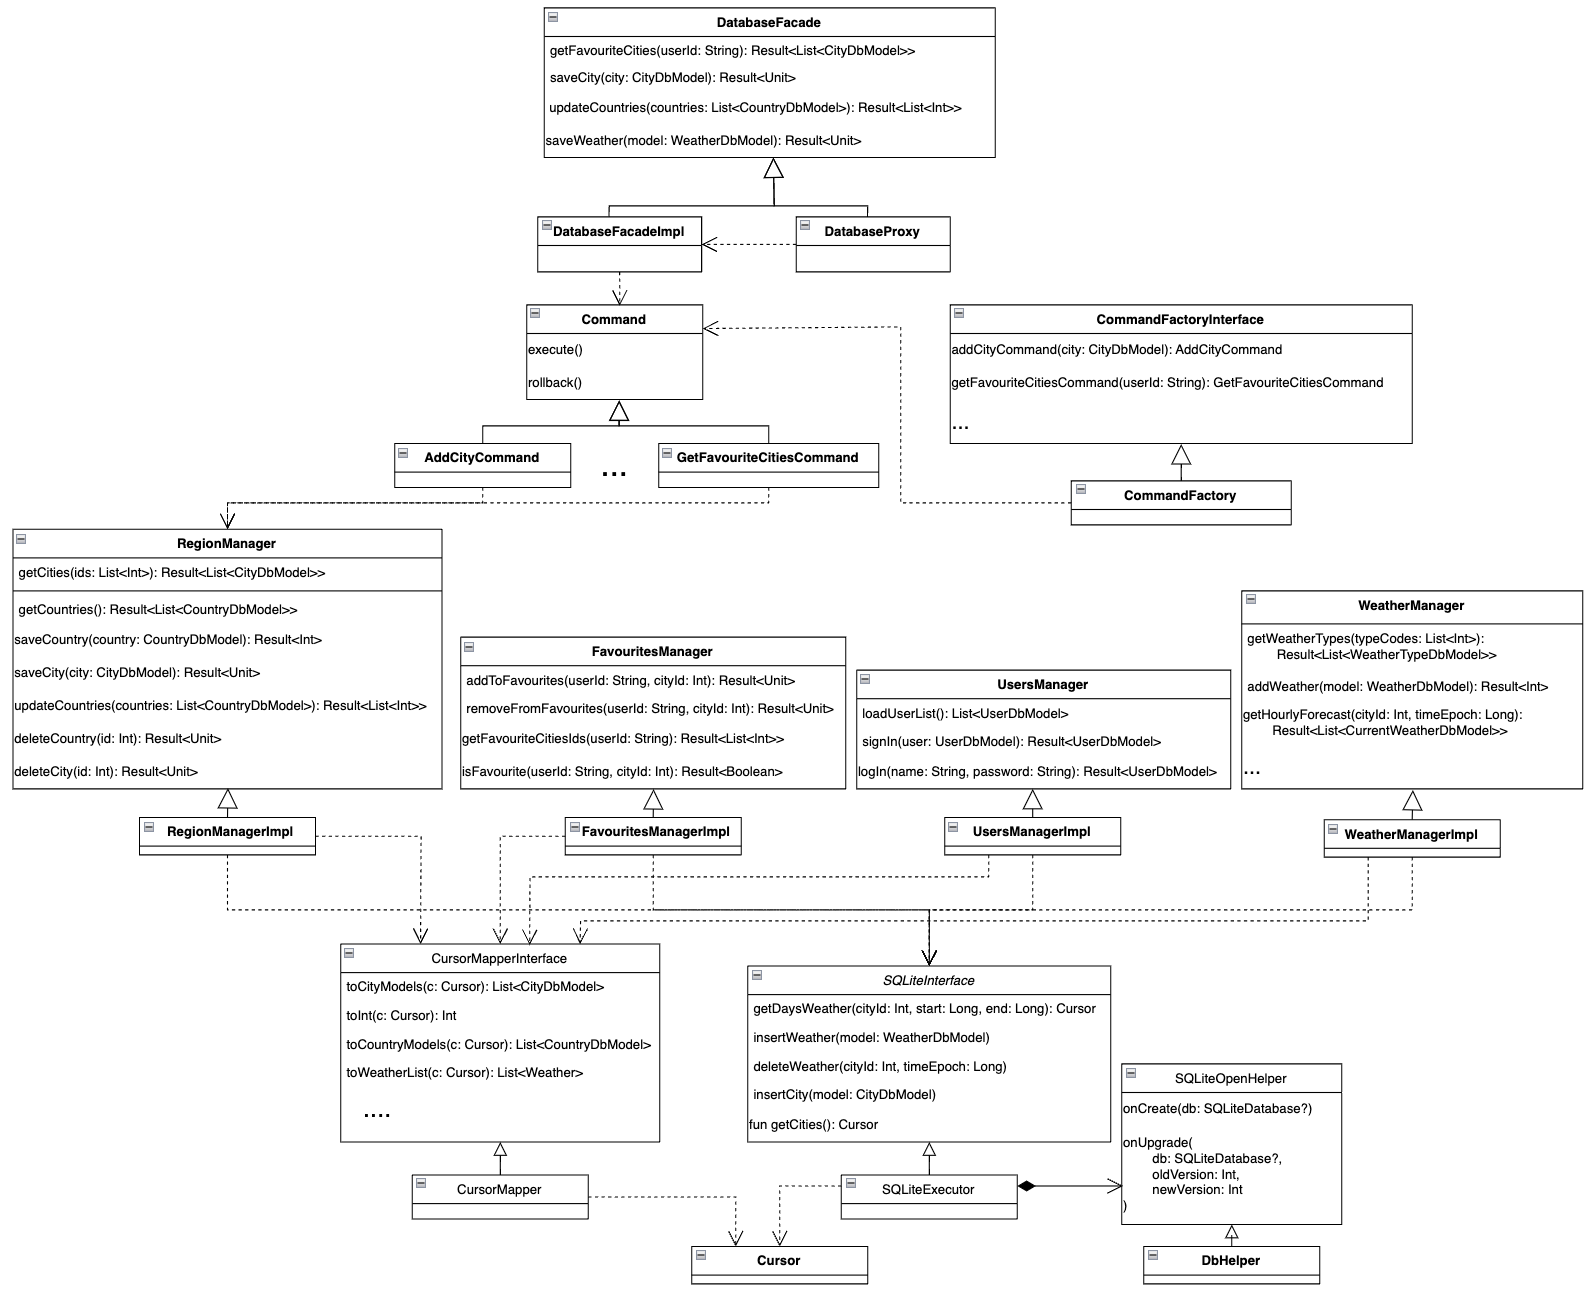
\includegraphics[width=\textwidth, height=0.65\textheight]{tools/img/db_uml.png}
	\caption{
        UML-диаграмма модуля базы данных
    }
	\label{fig:db_uml}
\end{figure}

\begin{table}[h!]
    \centering
    \begin{tabular} { | m{5cm} | m{10cm} | }
        \hline
            \textbf{Класс} & \textbf{Ответственность} \\
        \hline
            SQLiteInterface & Формирование и отправка SQL-запросов. \\
        \hline
            CursorMapperInterface & Чтение Cursor и формирование результата извлечения данных из БД. \\
        \hline
            WeatherManager & Реализация прецедентов, связанных с погодой. \\
        \hline
            UsersManager & Реализация прецедентов, связанных с пользователями. \\
        \hline
            RegionManager & Реализация прецедентов, связанных с регионами. \\
        \hline
            FavouritesManager & Реализация прецедентов избранного. \\
        \hline
            Command & Управление выполнением прецедентов: делегирование, кеширование результатов и отмена. \\
        \hline
            CommandFactory & Создание объектов Command. \\
        \hline
            DatabaseFacade & Унификация взаимодействия с базой данных. \\
        \hline
            DatabaseProxy & Реализация ролевой модели. \\
        \hline
            SQLiteOpenHelper & Библиотека для низкоуровневого взаимодействия с реляционной СУБД. \\
        \hline
            DatabaseProxy & Реализация ролевой модели. \\
        \hline
        \end{tabular}
    \caption{\centering Описание ответственностей основных классов модуля базы данных}
    \label{table:responsibility}
\end{table}

\subsection{Технологический стек приложения}
Погодное приложение удобнее всего использовать на мобильном устройстве.
Исходя из этого, для разработки выбрана операционная система Android, так как она является самой популярной среди всех ОС на мобильных устройствах~[9].
Далее следует выбрать системы управления выбранными базами данных.
В качестве локальной реляционной СУБД будет использоваться <<SQLite>>~[13], а в качестве документальной -- <<Firebase>>~[14].
Затем выбирается язык программирования.
Самый популярный и новый язык для разработки под Android -- Kotlin~[12].
Это типизированный и полностью объектно-ориентированный язык.
Он предоставляет все необходимые средства для реализации погодного приложения.
Для реализации графического интерфейса был выбран фреймворк <<Jetpack Compose>>~[15].
Он позволяет описывать интерфейс с помощью декларативного подхода и является самым популярным для создания графических интерфейсов на <<Android>>.
Также был выбран сервис <<Weather API>>~[19], предоставляющий погодные данные.


\subsection*{Схема взаимодействия с Firebase}
На рисунке~\ref{fig:interaction} изображена схема взаимодействия с СУБД Firebase.

\begin{figure}[H]
	\centering
	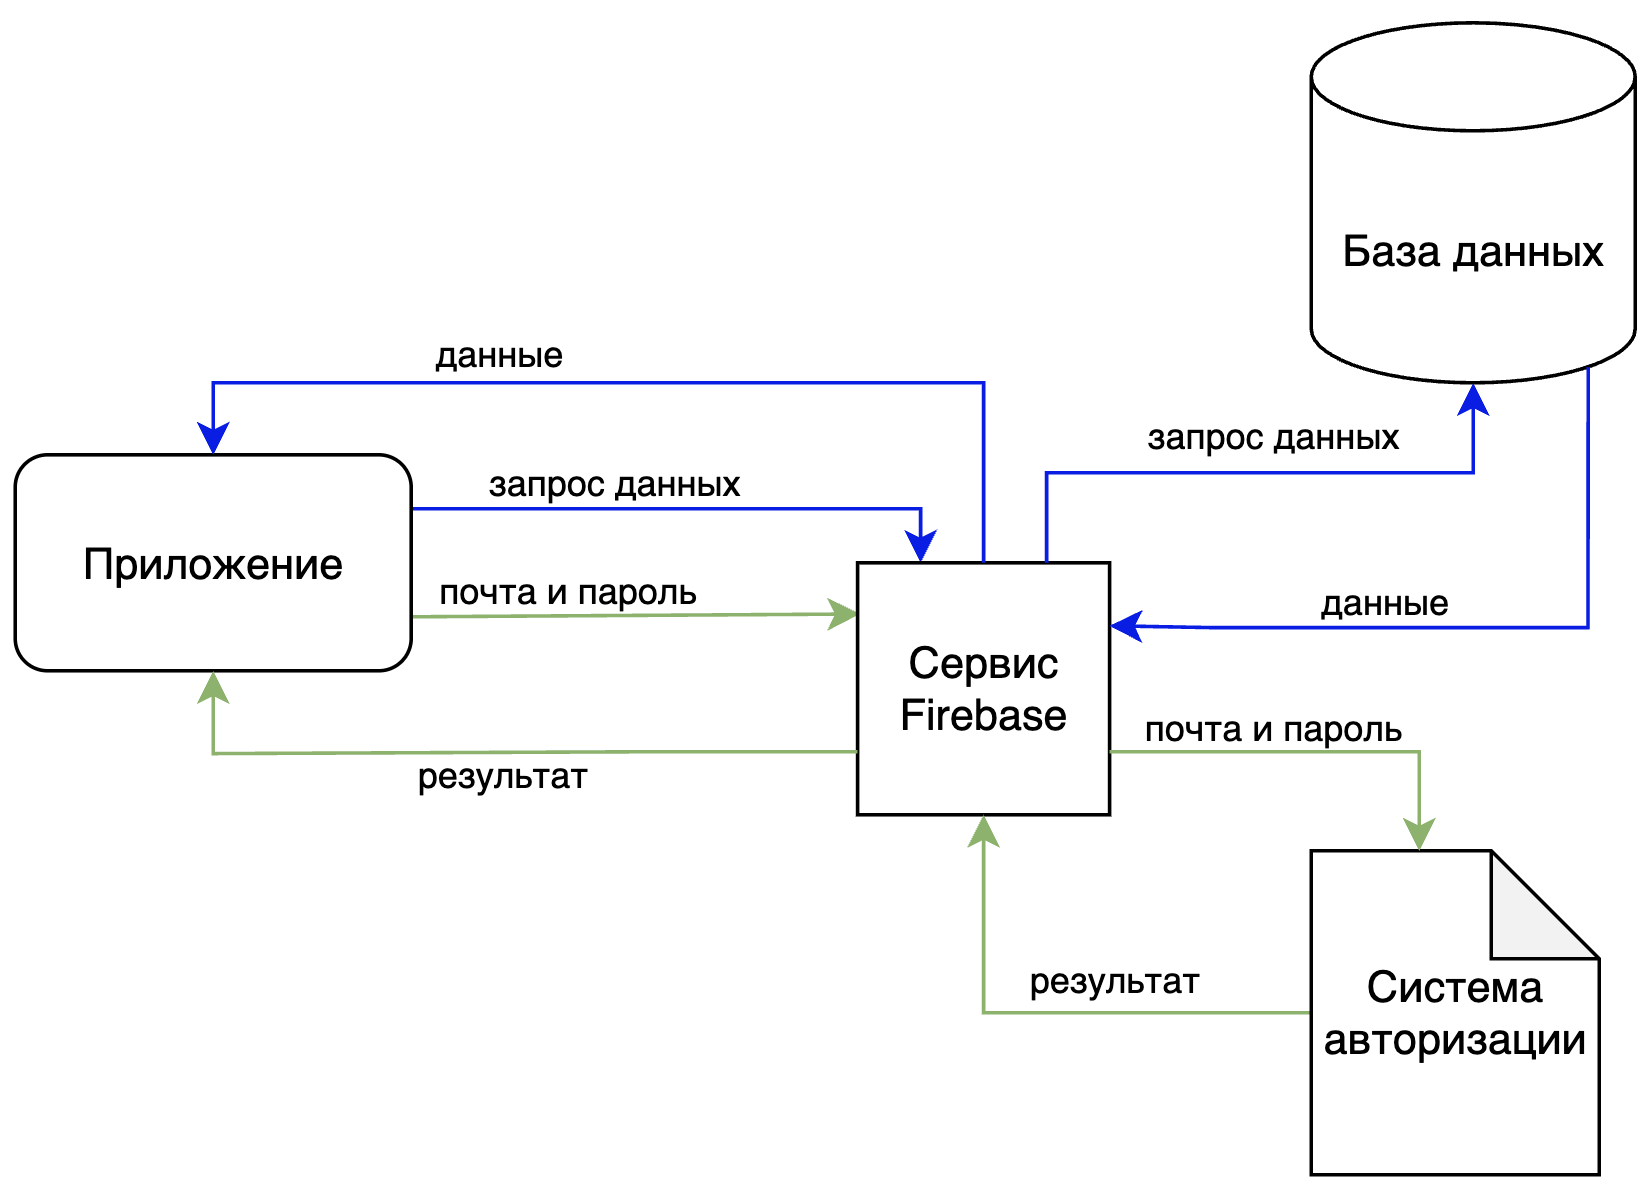
\includegraphics[height=0.22\textheight]{tools/img/interaction.png}
	\caption{
        Схема взаимодействия приложения и СУБД Firebase; зелёными стрелками показан поток данных для авторизации, а синими -- для чтения данных
    }
	\label{fig:interaction}
\end{figure}

\section{Реализация SQL-запросов к базе данных}
В листингах~\ref{lst:create}--\ref{lst:get} представлены все реализованные SQL-запросы для работы с базой данных.
\lstinputlisting[
    label = lst:create,
    caption = Реализация SQL-запросов для создания таблиц базы данных
] {code/create.sql}

\lstinputlisting[
    label = lst:delete,
    caption = Реализация SQL-запросов для удаления таблиц и данных
] {code/delete.sql}

\lstinputlisting[
    label = lst:insert,
    caption = Реализация SQL-запросов для добавления данных
] {code/insert.sql}

\lstinputlisting[
    label = lst:get,
    caption = Реализация SQL-запросов для извлечения данных
] {code/get.sql}

\section{Реализация взаимодействия с Firebase}
В листингах~\ref{lst:user}--\ref{lst:favourite} из приложения <<А>> представлена реализация взаимодействия с удалённой базой данных.
Прецеденты, реализованные в данных листингах:
\begin{itemize}
    \item регистрация пользователя;
    \item вход в аккаунт;
    \item добавление в избранное;
    \item удаление из избранного;
    \item получение списка городов, добавленных в избранное данным пользователем;
\end{itemize}
Все операции реализованы так, что поток их выполнения не блокируется.

\section{Методы тестирования базы данных}
Для того, чтобы протестировать базу данных, необходимо:
\begin{itemize}
    \item выделить классы эквивалентности для каждого прецедента;
    \item написать модульный тест для каждого класса эквивалентности.
\end{itemize}

\subsection{Классы эквивалентности}
В таблице~\ref{table:eqclass} представлены классы эквивалентности для каждого прецедента базы данных без учёта ролевой модели.

\begin{longtable}{ | m{65mm} | m{18em}| }
    \hline
        \textbf{Прецедент} & \textbf{Классы эквивалентности} \\
    \hline
        Вставить город & Вставить: 2 города из разных стран; 2 города из 1 страны; 2 одинаковых города. \\
    \hline
        Вставить страну & Вставить: 2 различные страны; 2 одинаковые страны.  \\
    \hline
        Вставить график & Вставить: пустой график; график с несколькими точками; уже вставленный график. \\
    \hline
        Удалить график & Удалить: не сохранённый график; сохранённый график. \\
    \hline
        Вставить тип погоды & Вставить: не сохранённый тип погоды; сохранённый тип погоды. \\
    \hline
        Вставить суточную погоду & Вставить: сохранённую погоду; не сохранённую погоду. \\
    \hline
        Вставить часовую погоду & Вставить: сохранённую погоду; не сохранённую погоду. \\
    \hline
    \endfirsthead
    
    \hline
        \textbf{Прецедент} & \textbf{Классы эквивалентности} \\
    \hline
    \endhead
    \endfoot
    \hline
        Вставить пользователя & Вставить: пользователя с именем без пробелов; пользователя с пробелами в именах; пользователя с не уникальным id. \\
    \hline
        Добавить в избранное  & Добавить: город из избранного; 2 города не из избранного из одной страны; 2 города не из избранного из разных стран. \\
    \hline
        Получить часовую погоду & Получить часовую погоду: за 1 день при её наличии в БД; за несколько дней при её наличии в БД; за 1 день при её отсутcтвии в БД; за несколько дней при её отсутствии в БД; за несколько дней при её частичном наличии в БД.  \\
    \hline
        Получить суточную погоду & Получить суточную погоду: за 1 день при её наличии в БД; за несколько дней при её наличии в БД; за 1 день при её отсутствии в БД; за несколько дней при её отсутствии в БД; за несколько дней при её частичном наличии в БД. \\
    \hline
        Удалить из избранного  & Удалить: город из избранного; город не из избранного; город из избранного, передав id другого пользователя. \\
    \hline
        Получить избранные города & Получить избранные города, когда: избранное пустое; в избранном несколько городов, сохранённых в БД; в избранном несколько городов, частично сохранённых в БД, в избранном 1 город, не сохранённый в БД. \\
    \hline
        Поиск города & Поиск города: запрос не пуст, БД не пуста и несколько результатов; запрос не пуст, БД не пуста и нет результатов; запрос не пуст, БД не пуста и 1 результат; запрос не пустой и БД пуста; запрос пустой и БД не пуста; запрос пустой и БД пуста. \\
    \hline
    \caption{
        \centering
        Классы эквивалентности для тестирования всех прецедентов базы данных без учёта ролевой модели, конец таблицы
     }
    \endlastfoot
    \caption{
        \centering
        Классы эквивалентности для тестирования всех прецедентов базы данных без учёта ролевой модели, начало таблицы
     }
     \label{table:eqclass}
 \end{longtable}

 \subsection{Модульное тестирование базы данных}
 В системе Android есть возможность написать модульный тест для какого-либо класса и запустить его в тестовом окружении~[16].
 Таким образом, аналог мобильного устройства и базы данных на нём будет доступен с помощью симуляции.
 Это делает возможным реализацию модульных тестов для базы данных, покрывающих каждый класс эквивалентности каждого прецедента.
 Модульные тесты должны быть независимы друг от друга и состоять из 3 частей:
 \begin{itemize}
     \item инициализация входных данных;
     \item выполнение определённого действия;
     \item проверка результата.
 \end{itemize}

В листинге~\ref{lst:test} представлен пример модульного теста, проверяющего работоспособность вставки сущности страны.
Тестом является метод тестового класса, помеченный аннотацией <<@Test>>.
Класс является тестовым, если он помещён в специальную директорию.
Тесты объединены в различные классов в зависимости их целей.
 \lstinputlisting[
    label = lst:test,
    caption = Модульный тест для проверки сохранения стран в базу данных
] {code/test.kt}

\section*{Выводы из технологической части}
В данном разделе был проведён выбор технологического стека приложения, выполнено проектирование модуля базы данных.
В результате получена реализация базы данных и погодного приложения.
Также были описаны методы тестирования модуля базы данных.